\documentclass[11pt]{article}
\usepackage{mathpaper}

\begin{document}
如图,在$\Delta ABC$中,$D$是线段$BC$上一点,满足$AB \bot AD$,若$AB=1$、$CD=4$、$\angle ABC=20^{\circ}$,求$\Delta ABC$的面积。
\begin{figure}[htb]
    \centering
    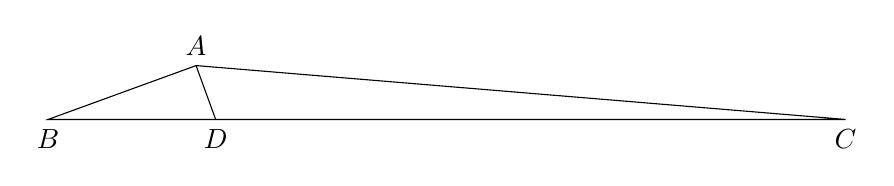
\begin{tikzpicture}[scale=2]
        \coordinate[label=below:{$D$}] (D) at (0,0);
        \coordinate[label=above:{$A$}] (A) at (-0.12447,0.34202);
        \coordinate[label=below:{$B$}] (B) at (-1.06417,0);
        \coordinate[label=below:{$C$}] (C) at (4,0);
        \draw (A)--(B)--(C)--cycle;
        \draw (A)--(D);
    \end{tikzpicture}
\end{figure}
\end{document}